\subsubsection{Memory Usage}

Charts on Figures \ref{fig:sequential_client_app_memory}, \ref{fig:parallel_client_app_memory}, \ref{fig:sequential_server_app_memory}, and \ref{fig:parallel_server_app_memory} represent the memory usage of clients and servers during sequential and parallel experiments.

\subsubsection*{Overall Application Client Memory Usage}

HTTP/1+TLS, HTTP/2 and HTTP/2+TLS managed to require more memory than HTTP/3 during parallel experiments. The latter remained as most costly during sequential experiments, however.

\subsubsection*{HTTP/1+TLS Memory Usage}

HTTP/1+TLS required more memory when performing parallel requests. HTTP/1 relies on TCP to manage its HTTP requests, resulting in a low memory consumption. Therefore, HTTP/1+TLS' memory usage is related to TLS' required features to be able to deliver encrypted data.

\subsubsection*{HTTP/2 Memory Usage}

HTTP/2 parallel requests managed to use a lot of memory when compared to sequential requests. HTTP/2 multiplexing control flow allocates buffers for each one of its streams \cite{rfc7540}. Thus, resulting in a large amount of allocated memory.

This behavior gets worse as payload size increase. It demands more space to be able to maintain all requests in the buffer while they are sent to the server. Therefore, this happens as the server cannot keep up with the data being transferred, taking longer to remove the HTTP request from the buffer. Consequently, the buffer grows even more, requiring more memory.

\subsubsection*{Overall Application Server Memory Usage}

While sequential server's memory usage remained similar to its client, parallel server's differs from its client.

HTTP/2 buffer did not impact as much as it did on its client. This buffer is used by the client to send data to the server. Thus, since the server only needs to respond requests that were sent by the client, it results in it never having to perform a large amount of concurrent requests.

Other than HTTP/2's memory usage, other protocols required approximately the same as its clients.

\subsubsection*{HTTP/3's Memory Usage}

HTTP/3's memory (Figure \ref{fig:parallel_client_app_memory}) usage was very similar to QUIC's (Figure \ref{fig:parallel_client_transport_memory}). Unlikely HTTP/2, QUIC only have UDP receive buffer, which in our case was 26MiB in size. Therefore, all of its memory usage is related cryptography, handling UDP packets, and maintaining its internal state.

Parallel requests memory usage was a bit higher when compared to sequential requests. Concurrent requests requires QUIC to maintain status and encrypt more requests than usual. For that reason it requires a bit more of memory.

\clearpage

\begin{figure}[h!]
    \centering
    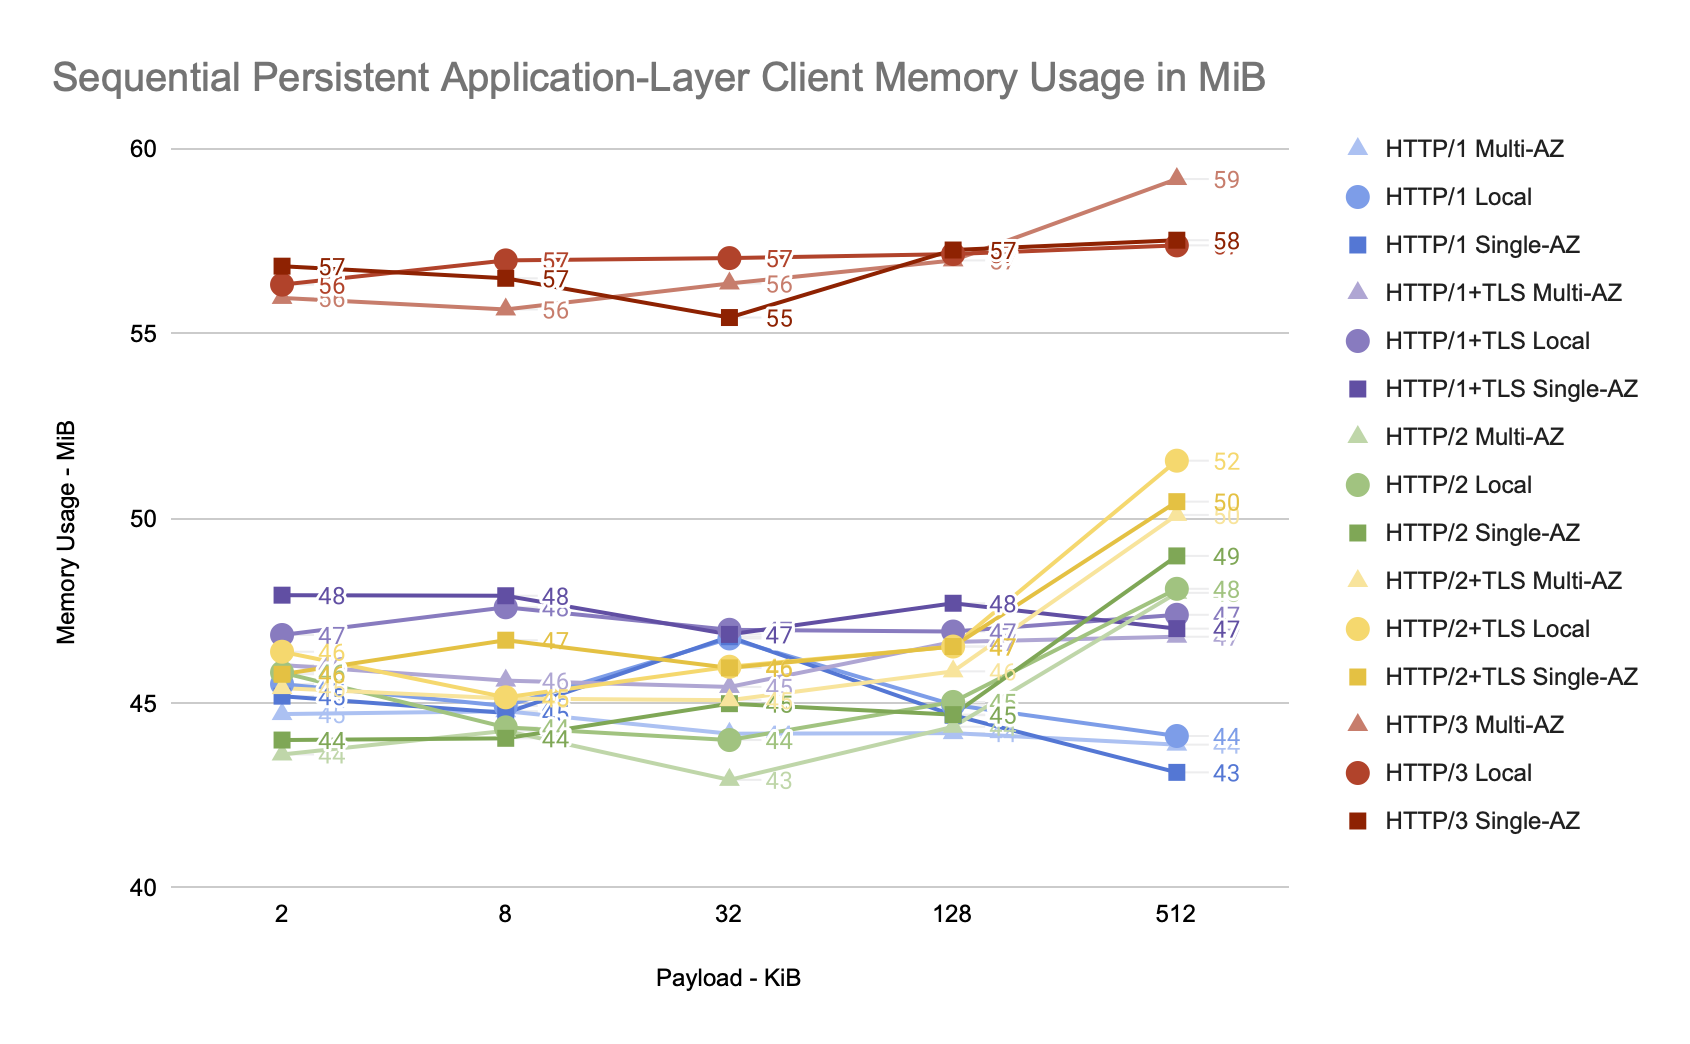
\includegraphics[width=\linewidth]{figures/charts/Sequential Persistent Application-Layer Client Memory Usage in MiB.png}
    \caption{Sequential Persistent Application-Layer Client Memory Usage in MiB}
    \label{fig:sequential_client_app_memory}
\end{figure}
\begin{figure}[h!]
    \centering
    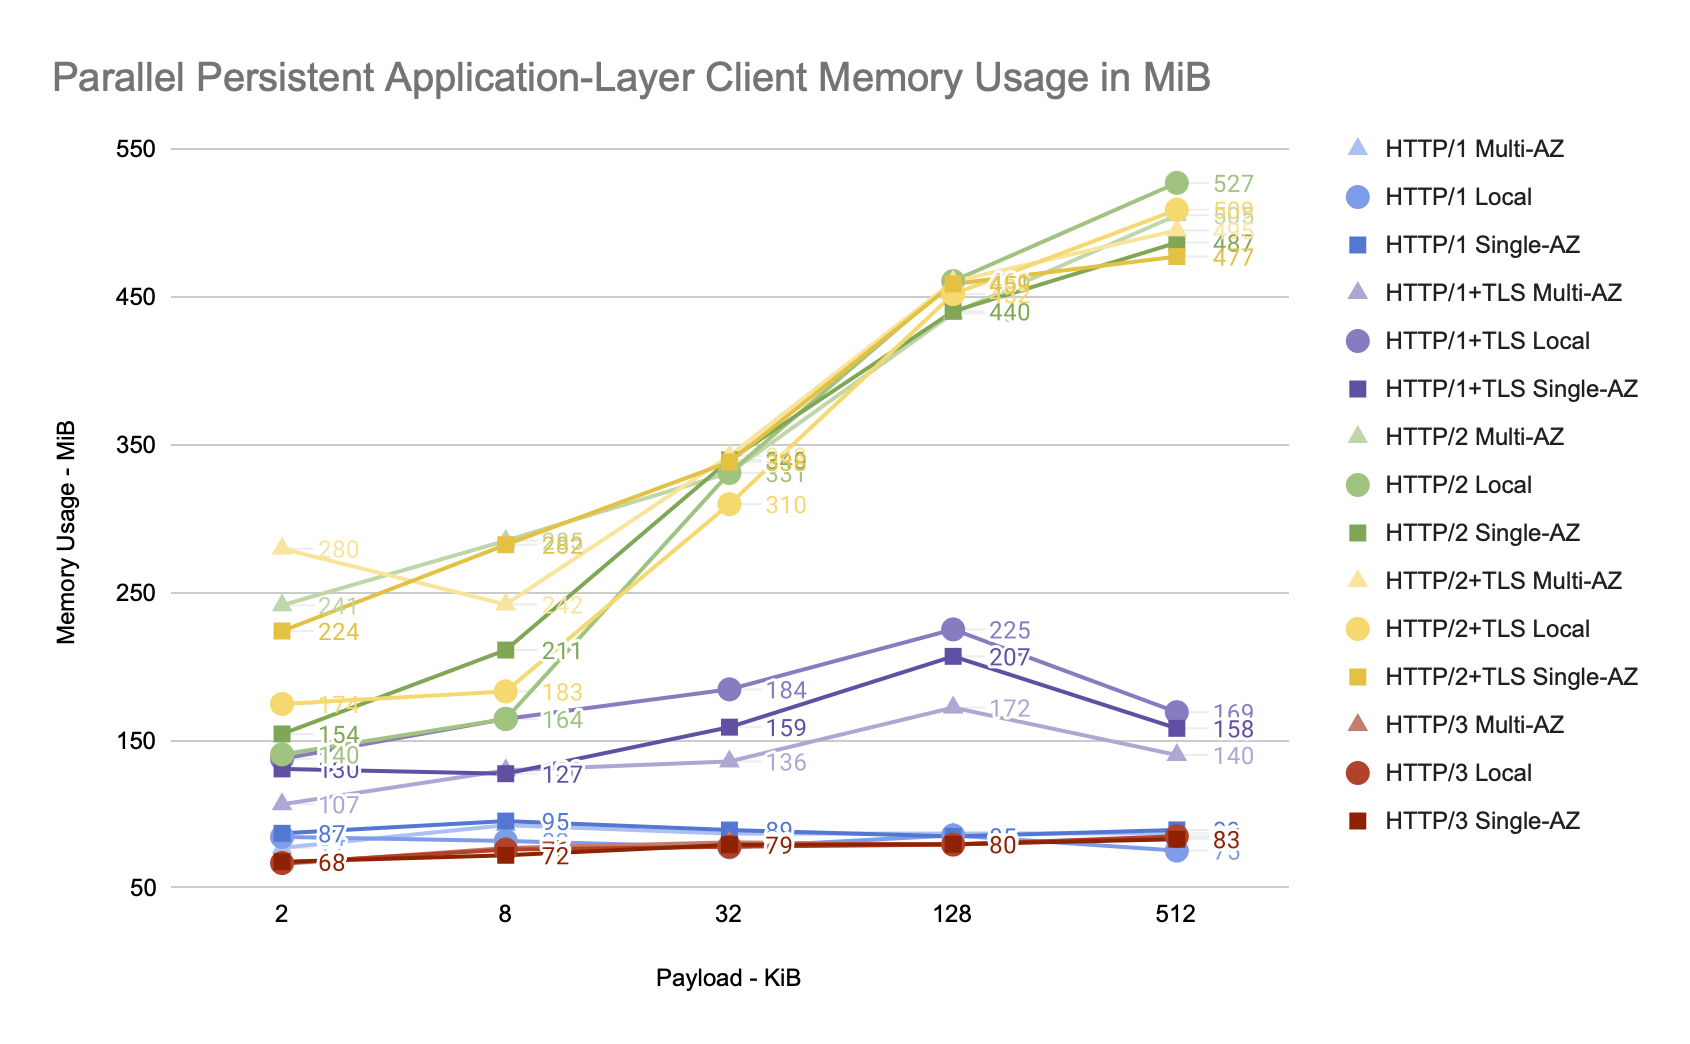
\includegraphics[width=\linewidth]{figures/charts/Parallel Persistent Application-Layer Client Memory Usage in MiB.png}
    \caption{Parallel Persistent Application-Layer Client Memory Usage in MiB}
    \label{fig:parallel_client_app_memory}
\end{figure}

\begin{figure}[h!]
    \centering
    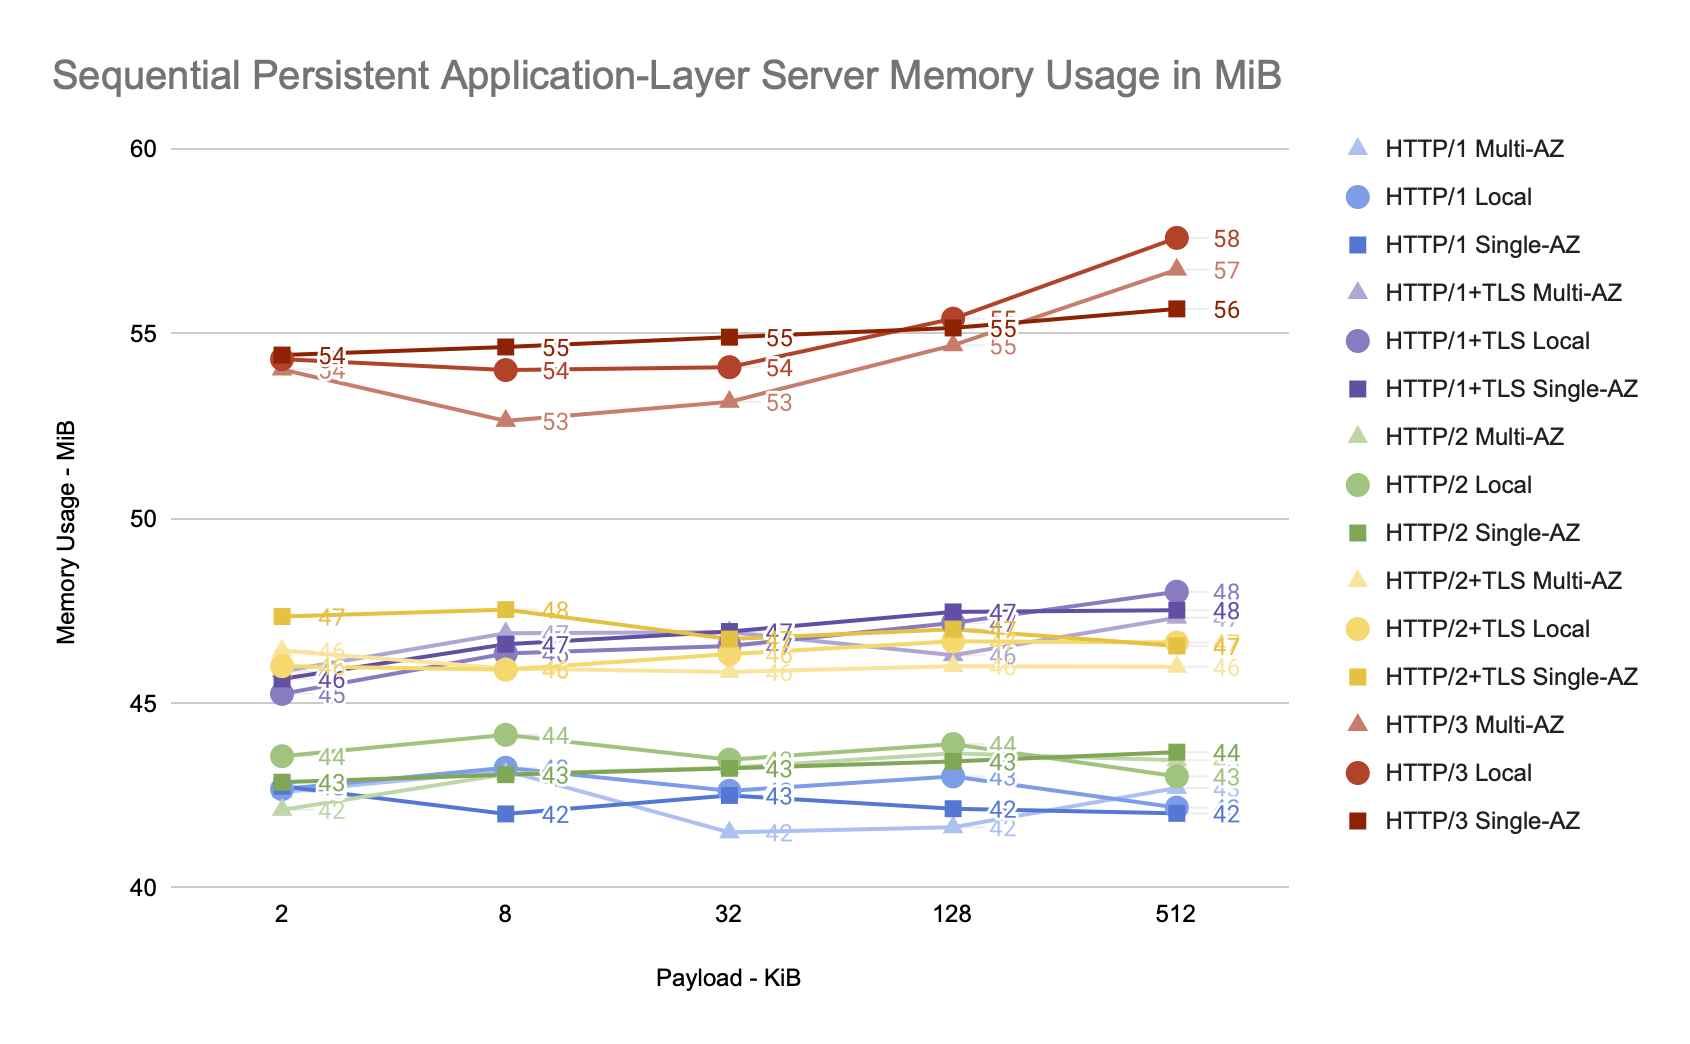
\includegraphics[width=\linewidth]{figures/charts/Sequential Persistent Application-Layer Server Memory Usage in MiB.png}
    \caption{Sequential Persistent Application-Layer Server Memory Usage in MiB}
    \label{fig:sequential_server_app_memory}
\end{figure}
\begin{figure}[h!]
    \centering
    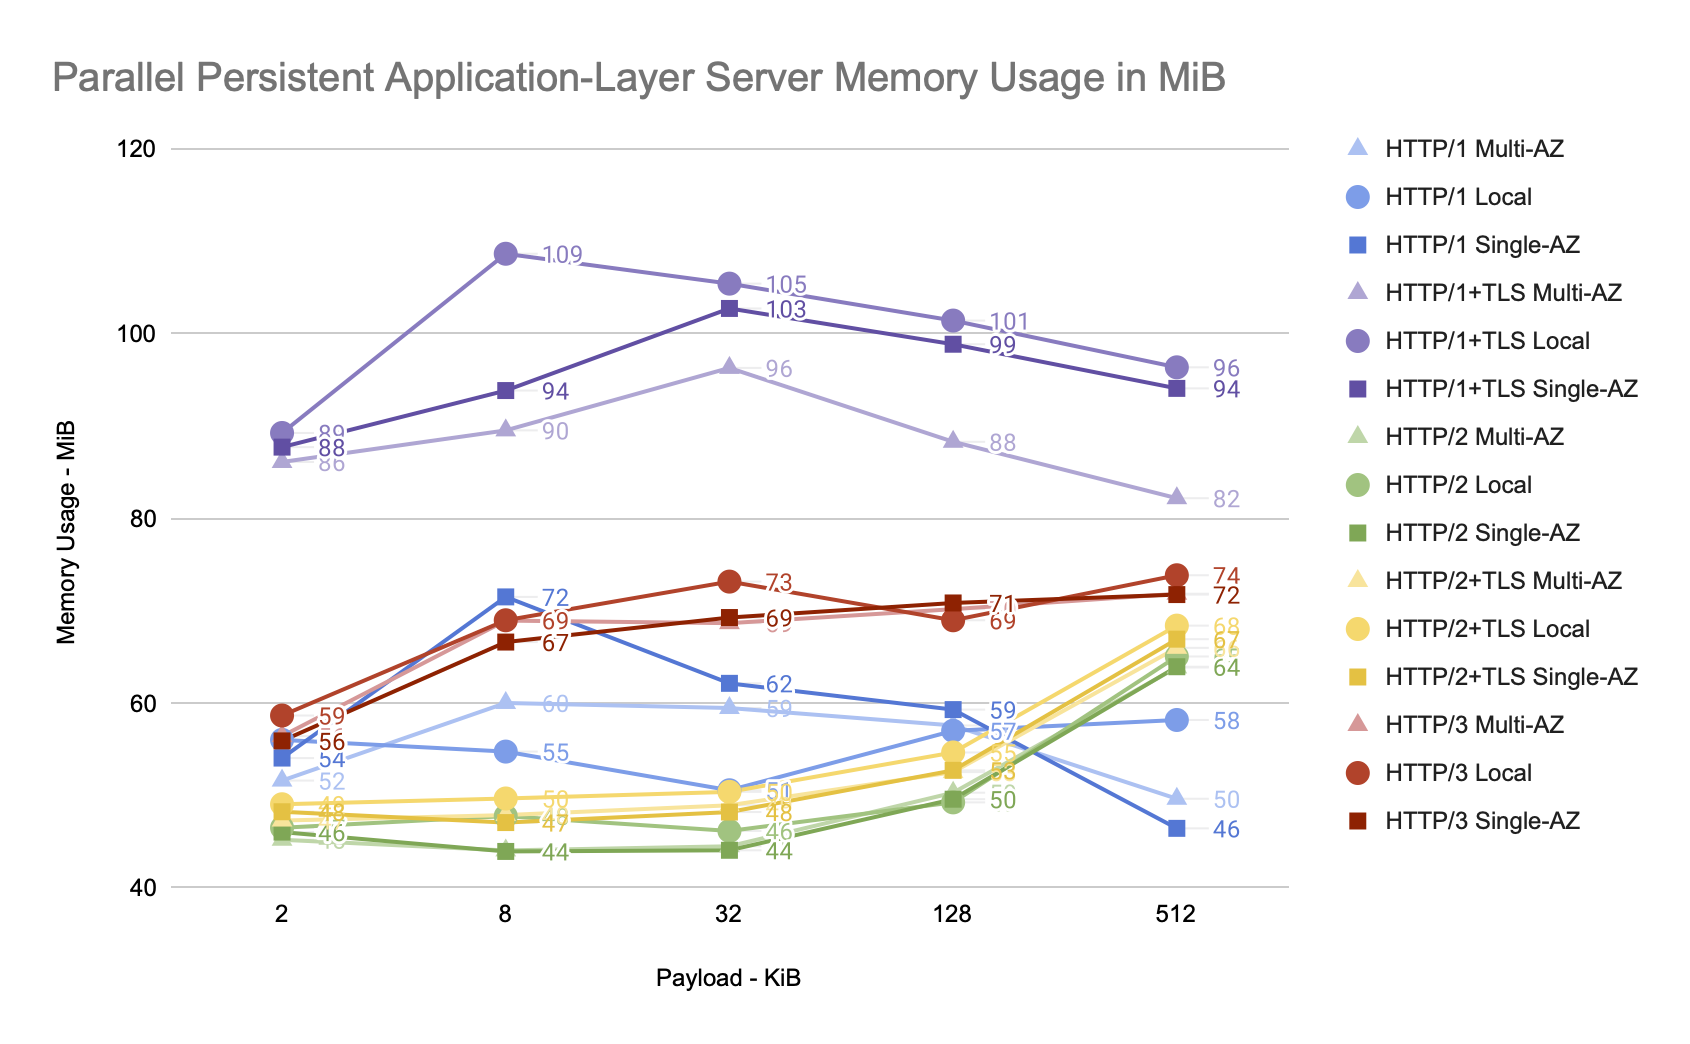
\includegraphics[width=\linewidth]{figures/charts/Parallel Persistent Application-Layer Server Memory Usage in MiB.png}
    \caption{Parallel Persistent Application-Layer Server Memory Usage in MiB}
    \label{fig:parallel_server_app_memory}
\end{figure}
